\documentclass[a4paper]{article}
\usepackage[pdftex]{graphicx}
\usepackage{anysize}
\marginsize{3cm}{3cm}{3cm}{3cm}
\linespread{1.2}
\usepackage[utf8]{inputenc}
\usepackage[T1]{fontenc}       
\usepackage[swedish]{babel}      
\usepackage{epstopdf}     % För svensk avstavning och svenska
\usepackage[osf]{mathpazo} % Palatino with smallcaps and oldstyle numbers
\usepackage[scaled]{helvet}
\usepackage{float}
\restylefloat{table}
\usepackage{etoolbox}

\newcommand\getcurrentref[1]{%
 \ifnumequal{\value{#1}}{0}
  {??}
  {\the\value{#1}}%
}  
\newcommand\requirement[2]{
	\numberedrow{Krav}{#1}{#2}
}
\newcommand\scenario[2] {
	\numberedrow{Scenario}{#1}{#2}
}
\newcommand\numberedrow[3]{
	\noindent
	\textbf{#1 \getcurrentref{section}.\getcurrentref{subsection}.#2.} #3
	
}

\usepackage{fancyhdr}
\fancyhf{}
\fancyhead[L]{Ansvarig: SG}
\fancyhead[C]{Datum: \today}
\fancyhead[R]{Version: 0.12}


\title{SRS - Software Requirements Specification: NewPussSystem}                  	
\author{Systemarkitektgruppen \\ Lars Gustafsson | Martin Lichota | Marcel Tovar Rascon}
\date{}

\begin{document}

\maketitle
\thispagestyle{fancy}
\tableofcontents
\newpage

\section*{Dokumenthistorik}

\begin{tabular}{ l l l l }
Ver. & Datum & Ansv. & Beskrivning \\\hline
0.1 & 8 november 2014 & SG & Struktur för dokumentet\\
0.2 & 10 november 2014 & SG & Lägga till krav från UG\\
0.3 & 11 november 2014 & SG & Revidera krav samt ändra struktur\\
0.4 & 12 november 2014 & SG & Lade till nya samt reviderade krav\\
0.5 & 12 november 2014 & SG & Lade till nya samt reviderade krav\\
0.6 & 12 november 2014 & SG & Lade till nya samt reviderade krav\\
0.7 & 12 november 2014 & SG & Lade till nya samt reviderade krav\\
0.8 & 12 november 2014 & SG & Lade till nya samt reviderade krav\\
0.9 & 12 november 2014 & SG & Reviderade krav samt lade till scenarion\\
0.10 & 13 november 2014 & SG & Skapade scenarion för projektledning.\\
0.11 & 13 november 2014 & SG & Skapade scenarion för tidrapportmall och lade till krav.\\
0.12 & 14 november 2014 & SG & Administration och tidrapportering är klart.\\

\end{tabular}
\section{Inledning}       


Dokumentet beskriver kraven för <Program X>, ett tidsrapportingssystem för projekt som diverse användare kan logga in på.

\section{Referensdokument}
I denna version används inget referensmaterial.
\section{Bakgrund och mål}   
\subsection{Huvudmål}
Huvudmålet är att tillhandhålla ett system där olika användare, såsom projektledare och övriga projektmedlemmar, skall kunna tidsrapportera och loggföra det fortgående arbetet i sitt projekt. 

\subsection{Aktörer och deras mål}
Följande aktörer kommer att använda systemet:
\begin{itemize}
\item [] \textbf{Användare} En vanlig användare kan logga in och ut ur systemet. Användaren kan erhålla en specifik roll (se nedan).
\item [] \textbf{Projektmedlem(t1, t2, t3) }En användare kan tilldelas rollen som projektmedlem. Denne kan tidrapportera och har även tillgång till historik rörande den egna samt gruppens totala tidrapportering.
\item [] \textbf{Projektledare} En användare kan tilldelas rollen som projektmedlem vilket ger den administrativa rättigheter för ett givet projekt. En projektledare kan tillsätta vanliga användare en projektmedlemsroll. Denne kan deltaga i en projektgrupp och har utöver sina befogenheter tillgång till samma funktionaliteter som en projektmedlem.
\item [] \textbf{Administratör} En administratör är en och endast en användare som har befogenheter att lägga till och ta bort andra användare. Administratören tillsätter även projektledare och skapar projektgrupper. Administratören kan inte deltaga i en projektgrupp men har utöver detta samma priviligerade rättigheter som projektledare.
\end{itemize}

\section{Terminologi}
Här följer ord och uttryck som används i rapporten och är till för att öka förståelsen.
\begin{itemize}
\item [Användarnamn] Unik indentifikationsfras för att representera en användare i systemet..
\item [Lösenord] Hemlig fras endast känd för var unik användare samt systemet så användaren kan påvisa sin identitet.
\item [Inloggad] En användare som har identifierat sig mot systemet med användarnamn och lösenord, detta sker genom att användaren loggar in.
\item [Logga in] Se inloggad.
\item [Användarstatus] En indikation på var användare som avgör hur vida den får logga in eller ej.
\item [Projektgrupp] En grupp bestående av vanliga användare och projektledare.
\item [Tidsrapport] En rapport som innehåller arbetsbelasting för en användare under en fix tidsperiod bundet till en specefik projektgrupp.
\item [Huvudsida] Med huvudsida avses den första vyn som användaren blir dirigerad till direkt efter inloggning. 
\item [Användarlista] En lista med alla användarnamn och lösenord som är sparade i databasen.
\item [Aktivitetsruta] Cellen där aktivitet (raden) och subaktivitet (kolumnen) möts.
\item [Information] Med information avses t.ex. användare, projekt eller tidrapporter.
\end{itemize}
\section{Kontextdiagram}
Denna version innehålller inte ett kontextdiagram.
\section{Funktionella krav}
\subsection{Generella krav}
\label{krav-funk-gen}

\requirement{1}{En användare kan vara projektmedlem i en och endast en projektgrupp åt gången.}
\requirement{2}{Maximalt 50 användare kan vara inloggade på systemet samtidigt.}
\requirement{3}{Samtliga användare skall ha tillgång till följande funktionaliteter: start, tidrapportering, projektinformation, byta lösenord, hjälp samt utloggning.}
\requirement{4}{Samtliga funktionaliter i krav \ref{krav-funk-gen}.3 skall vara tillgängliga i menyn.}
\requirement{5}{Projektledarna har tillgång till projektadministrationsfunktionaliter. Det listas som ''projektadministration'' och finns tillgängligt för dessa i menyn.}
\requirement{6}{Administratören har tillgång till administrationsfunktionaliteter. Det listas som ''administration'' och finns tillgängligt för denne i dess meny.}
\requirement{7}{Administrationsfunktionaliteter avser även projektadministration och därmed har administratörer, utöver sina priviligerade rättigheter, även projektledarnas befogenheter.}
\requirement{8}{Menyn, oavsett typ av användare, skall vara tillgänglig på samtliga sidor som visas av systemet.}
\requirement{9}{En projektgrupp skall bestå av 1-20 användare.}
\requirement{10}{Varje borttagning av information skall bekräftas av en dialogruta frågandes om man är säker. Om användaren väljer ''Ja'', tas informationen bort och användaren kommer tillbaka till en uppdaterad sida med informationen. Om ``Nej'' väljs, går användaren tillbaka till nuvarande sida.}
\requirement{11}{Det finns sammanlagt fem roller i systemet: administratör, projektledare, t1, t2, t3.}
\requirement{12}{Det skall finnas en administratör (se krav \ref{krav-funk-admin}.2) i systemet. I varje projektgrupp får det finnas 1-2 projektledare (se krav \ref{krav-funk-proj}.1) och de tre teamen, t1, t2 och t3 (se krav \ref{krav-funk-gen}.13).}
\requirement{13}{I t1, t2 och t3 får det finnas 1-6 användare/team, alltså sammanlagt 1-18 användare.}
\requirement{14}{Administratören kan ej deltaga i en projektgrupp.}


\subsection{Autentisering}
\label{krav-funk-aut}
\requirement{1}{För varje användare kan loginstatus antingen vara inloggad eller inte inloggad.}
\requirement{2}{Systemet skall hålla loginstatus i en serversession.}

% ----------------------- SCENARIO

\begin{table}[H]
\begin{tabular}{ | p{2cm} p{11cm} | }
   
        \hline
	\multicolumn{2}{|p{13cm}|}{ \indent\scenario{1}} \\
    \textbf{Syfte} & Logga in användaren i systemet.\\
    \textbf{Trigger} & Användaren inkommer till systemet. \\
    \textbf{Förutsättning} & Användaren är inte inloggad.\\
    \hline

	\multicolumn{2}{|p{13cm}|}{ \textbf{Subuppgifter}:} \\

	\multicolumn{2}{|p{13cm}|}{ 1. Användaren får datafält för användarnamn och lösenord.}\\
	\multicolumn{2}{|p{13cm}|}{ 2. Användaren matar in användarnamn och lösernord och skickar data till servern genom ``Logga in''-knappen.} \\	
	\multicolumn{2}{|p{13cm}|}{ 3. Användarens loginstatus ändras till inloggad och är dirigerad till huvudsidan. }\\ \hline
    \multicolumn{2}{|p{13cm}|}{ \textbf{Varianter}: }\\
	\multicolumn{2}{|p{13cm}|}{ 3.a Det givna användarnamnet och lösernordet matchar inte något par i systemets databas. Detta meddelas då till användaren som får repetera inloggningen.}\\
	    \hline


\end{tabular}
\end{table}
% ----------------------- /END

\requirement{3}{När en användare når systemet och inte är inloggad skall denne få en förfrågan om användarnamn och lösenord.}
\requirement{4}{När en användare skickar ett användarnamn och lösenord skall dessa parametrar jämföras med användarlistan och om användaren skall få tillgång till systemet , så skall serverstatus ändras till ``inloggad'' och huvudsidan skall visas.}
\requirement{5}{Ingen annan information utöver inloggningsrutan skall visas för en inte inloggad användare.}


% ----------------------- SCENARIO
\begin{table}[H]
\begin{tabular}{ | p{2cm} p{11cm} | }
   
        \hline

    \multicolumn{2}{|p{13cm}|}{ \indent\scenario{2}} \\
    \textbf{Syfte} & Logga ut användaren från servern.\\
    \textbf{Trigger} & Användaren vill logga ut. \\
    \textbf{Förutsättning} & Användaren är inloggad.\\
    \hline
	\multicolumn{2}{|p{13cm}|}{ \textbf{Subuppgifter}:} \\
	\multicolumn{2}{|p{13cm}|}{ 1. Användaren väljer logga ut länken i menyn och loggas ut, samt dirigeras till en sida där utloggningen bekräftas.}\\ \hline
    \multicolumn{2}{|p{13cm}|}{\textbf{Varianter}: }\\
	\multicolumn{2}{|p{13cm}|}{1.a Användaren har redan blivit utloggad från servern. I sådana fall meddelas detta till användaren som dirigeras till utloggningssidan.} \\
	    \hline


\end{tabular}
\end{table}
% ----------------------- /END


\requirement{6}{Om en inloggad användare är inaktiv i längre än 20 minuter skall sagda användare loggas ut och tvingas att logga in igen innan fortsatt användning av systemet.}
\requirement{7}{Ett användarkonto kan endast vara inloggat på en enhet åt gången.}
\requirement{8}{Om en användare försöker logga in med ett användarkonto som redan är inloggat på en annan enhet, kommer den nya inloggingen att genomföras medan den andra enheten loggas ut.}
\requirement{9}{Scenario \ref{krav-funk-aut}.1 skall stödjas av systemet.}
\requirement{10}{Scenario \ref{krav-funk-aut}.2 skall stödjas av systemet.}
\subsection{Data}
\label{krav-funk-data}
\requirement{1}{Användarnamn skall bestå av 5-10 tecken, ascii (decimal) värden 48-57, 65-90, och 97-122 är tillåtna.}
\requirement{2}{Användarnamn måste vara unika.}
\requirement{3}{Lösenord skall bestå av sex tecken, ascii (decimal) värden 97-122 är tillåtna.}
\noindent\rule{8cm}{0.4pt} \\ %-------------------------------------------------------------------------------------
\requirement{4}{Tidrapportering sker i antal minuter.}
\requirement{5}{Tidrapportens utseende, med avseende på vilka aktiviteter man kan föra in tidinformation i, bestäms av administratören innan projektgruppen har skapats. När projektet är skapat skall det inte gå att ändra tidrapportens utseende.}
\requirement{6}{Tidrapportens grundmall skall innehålla information om användarnamn, projektgruppsnamn, datum och veckonummer. Det skall även tydligt framgå om den är signerad eller ej. Grundmallen genereras automatiskt av systemet.}
\requirement{7}{Samtliga tidrapportmallar sparas på servern.}
\requirement{8}{Maximalt 20 mallar kan lagras samtidigt, efter uppnådd maxgräns skrivs de över enligt FIFO-principen.}
\requirement{9}{En tidrapportmall ska bestå av 1-10 rader samt 1-5 kolumner som det går att mata in tidinformation i.}
\requirement{10}{Namnet på tidrapportmallen ska bestå av 5 tecken, ascii (decimal) värden 48-57 och 97-122 är tillåtna.}
\requirement{11}{Namnet på aktivitet och subaktivitet ska bestå av 3-5 tecken respektive 1 tecken, ascii (decimal) värden 48-57 och 97-122 är tillåtna.}
\requirement{12}{Tidinformationen får innehålla 1-5 tecken per aktivitetsruta, ascii (decimal) värden 48-57.}
\requirement{13}{Tidrapportmallarnas namn måste vara unika.}

\noindent\rule{8cm}{0.4pt}  %------------------------------------------------------------------------------------------------------

\requirement{14}{Ett projektgruppsnamn ska bestå av 5-10 tecken, ascii (decimal) värden 48-57 och 97-122 är tillåtna.}
\requirement{15}{Projektgruppsnamn måste vara unika.}

\noindent\rule{8cm}{0.4pt}  %------------------------------------------------------------------------------------------------------

\requirement{16}{Veckonumret får innehålla 1-2 tecken, ascii (decimal) värden 48-57}

\noindent\rule{8cm}{0.4pt}  %------------------------------------------------------------------------------------------------------

\requirement{17}{Det skall gå att lagra 1-100 tidrapporter/användare. Efter uppnådd maxgräns skrivs de över enligt FIFO-principen.}

\subsection{Administration}
\label{krav-funk-admin}

\begin{figure}[h!]
  \centering
    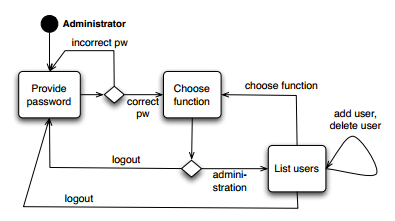
\includegraphics[width=0.5\textwidth]{admin_usage}
   \caption{A picture of a gull.}
   \label{image_admin_usage}
\end{figure}
\requirement{1}{Systemet ska stödja sekvensen för administrören som visas i Figur \ref{image_admin_usage}.}
\requirement{2}{Det skall finnas en och endast en administratör med användarnamnet ''admin'' och lösenordet ''adminpw''.}
\requirement{3}{Som inloggad administratör skall det vara möjligt att välja administrationsvyn på huvudsidan.}
\requirement{4}{En ny användare, skapad av administratören, måste ha ett unikt användarnamn samt bli tilldelad ett slumpmässigt lösenord från systemet.}
\requirement{5}{Om administratören försöker att lägga till en användare med ett användarnamn som redan existerar i systemet, skall användaren inte läggas till och ett felmeddelande skall visas.}
\requirement{6}{Om en administratör väljer administrationsvyn skall denne få åtkomst till administationsverktygen, men om samma val görs av en ickeadministratör skall denne istället få åtkomst till huvudsidan.}
\requirement{7}{I administrationsvyn skall alla användare listas med både användarnamn och lösenord.}
\requirement{8}{I administrationsvyn skall det vara möjligt att ta bort vilken användare som helst förutom administratören.}
\requirement{9}{Varje borttagning av användare ska bekräftas med en dialogrutan beskriven i krav \ref{krav-funk-gen}.10.}
\requirement{10}{I administrationsvyn skall det vara möjligt att lägga till en ny användare.}
\requirement{11}{Om en administratör försöker lägga till en ny användare med ett användarnamn som strider mot krav \ref{krav-funk-data}.1-2 skall ett felmeddelande visas och användaren skall inte läggas till.}

\noindent\rule{8cm}{0.4pt} %-----------------------------------------------------------------------------------------

\requirement{12}{Endast administratören skall kunna skapa projektgrupper i systemet.}
\requirement{13}{Endast administratören skall kunna tilldela projektmedlemmar en projektledarroll.}
\requirement{14}{Endast administratören skall kunna lägga till eller ta bort projektmedlemmar i ett projekt.}
\requirement{15}{Endast administratören skall kunna ta bort projektgrupper ur systemet.}
\requirement{16}{Administratören skall kunna utforma en tidrapportmall. Se även krav \ref{krav-funk-data}.5 och \ref{krav-funk-data}.6.}
\requirement{17}{Scenario \ref{krav-funk-admin}.1 - \ref{krav-funk-admin}.4 skall stödjas av systemet.}

%--------------SCENARIO

\begin{table}[H]
\begin{tabular}{ | p{2cm} p{11cm} | }
    \hline
    
    \multicolumn{2}{|p{13cm}|}{ \indent\scenario{1}} \\
    \textbf{Syfte} & Skapa projektgrupp.\\
    \textbf{Trigger} & Användaren vill skapa en projektgrupp. \\
    \textbf{Förutsättning} & Användaren måste vara inloggad som administratör.\\
    \hline

	\multicolumn{2}{|p{13cm}|}{\textbf{Subuppgifter}:} \\

	\multicolumn{2}{|p{13cm}|}{1. Användaren väljer att skapa projektgrupp.}\\
	\multicolumn{2}{|p{13cm}|}{2. Användaren väljer därefter tidrapportmall (se scenario \ref{krav-funk-admin}.4).}\\
	\multicolumn{2}{|p{13cm}|}{3. Denne får nu fylla i ett projektgruppsnamn och trycker därefter på ''OK''.} \\	
	\multicolumn{2}{|p{13cm}|}{4. Denne möts av en lista över användare i systemet. Första användaren som läggs till tilldelas automatiskt en projektledarroll.} \\	
	\multicolumn{2}{|p{13cm}|}{5. Användaren kan därefter lägga till fler projektgruppsmedlemmar. Det ska även vara möjligt att tilldela ytterligare en projektgruppsmedlem, en projektledarroll. När användaren är klar trycks ''OK''} \\	
	\multicolumn{2}{|p{13cm}|}{6. Projektgruppen skapas och användaren dirigeras till en sida som bekräftar detta. } \\	
	\hline
    \multicolumn{2}{|p{13cm}|}{\textbf{Varianter}: }\\
    \multicolumn{2}{|p{13cm}|}{4a. Projektgruppsnamnet existerar redan (se krav \ref{krav-funk-data}.15), användaren informeras och skickas tillbaka till steg 3.}\\
    \multicolumn{2}{|p{13cm}|}{4b. Projektgruppsnamnet strider mot krav \ref{krav-funk-data}.14. Användaren informeras och skickas tillbaka till steg 3.}  \\
    \multicolumn{2}{|p{13cm}|}{4c. Användaren får felmeddelande eftersom inga fler användare existerar. Denne informeras om detta och skickas tillbaka till huvudsidan.}\\
       \multicolumn{2}{|p{13cm}|}{5a. Användaren ska informeras om att det inte finns fler användare att lägga till i projektgruppen och få möjlighet att skickas till steg 7.}\\
    \multicolumn{2}{|p{13cm}|}{5b. Användaren ska informeras om någon av grupperna har max antal användare (se krav \ref{krav-funk-gen}.12 och \ref{krav-funk-gen}.13). Denne ska inte ha möjlighet att lägga till fler projektmedlemmar i den nämnda gruppen.}\\

    \hline
\end{tabular}
\end{table}

% ----------------------- /END



%--------------SCENARIO

\begin{table}[H]
\begin{tabular}{ | p{2cm} p{11cm} | }
    \hline
    
    \multicolumn{2}{|p{13cm}|}{ \indent\scenario{2}} \\
    \textbf{Syfte} & Lägga till/ändra roll på projektmedlem i projektgrupp.\\
    \textbf{Trigger} & Användaren vill lägga till eller ändra projektmedlemmens roll. \\
    \textbf{Förutsättning} & Användaren måste vara inloggad som administratör.\\
    \hline

	\multicolumn{2}{|p{13cm}|}{\textbf{Subuppgifter}:} \\

	\multicolumn{2}{|p{13cm}|}{1. Användaren väljer ''redigera projektmedlemmar''.}\\
	\multicolumn{2}{|p{13cm}|}{2. Användaren får upp en lista med samtliga projektgrupper och eventuella projektmedlemmar och en lista med samtliga användare i systemet som inte är projektmedlemmar överhuvudtaget.}\\
	\multicolumn{2}{|p{13cm}|}{3. Användaren har nu möjlighet att flytta över projektmedlemmar och icke projektmedlemmar till olika projektgrupper. Denne kan även ange vilken roll som projekt-medlemmen eller -medlemmarna ska ha.} \\	
	\multicolumn{2}{|p{13cm}|}{4. Användaren bekräftar genom att trycka ''OK''. Denne dirigeras till en sida med den nya informationen samt en bekräftelse.} \\	
	\hline
    \multicolumn{2}{|p{13cm}|}{\textbf{Varianter}: }\\
    \multicolumn{2}{|p{13cm}|}{1a. Det existerar inga projektgrupper/projektmedlemmar. Användaren informeras om detta och skickas tillbaka till huvudsidan.}\\
    \multicolumn{2}{|p{13cm}|}{4a. Användaren får felmeddelande då denne försökt att flytta över en projektledare som är den enda i sin projektgrupp. Denne ombedes att tillsätta en ny projektledare i gruppen innan förflyttning kan äga rum. Användaren dirigeras till steg 3.} \\
    \multicolumn{2}{|p{13cm}|}{5b. Användaren ska informeras om någon av grupperna har max antal användare (se krav \ref{krav-funk-gen}.12 och \ref{krav-funk-gen}.13). Denne ska inte ha möjlighet att lägga till fler projektmedlemmar i den nämnda gruppen. Användaren skickas tillbaka till steg 3.}\\

    \hline
\end{tabular}
\end{table}

% ----------------------- /END



%--------------SCENARIO

\begin{table}[H]
\begin{tabular}{ | p{2cm} p{11cm} | }
    \hline
    
    \multicolumn{2}{|p{13cm}|}{ \indent\scenario{3}} \\
    \textbf{Syfte} & Ta bort projektmedlemmar eller projektgrupp.\\
    \textbf{Trigger} & Användaren väljer ta bort projektgrupp/projektmedlemmar. \\
    \textbf{Förutsättning} & Användaren måste vara inloggad som administratör.\\
    \hline

	\multicolumn{2}{|p{13cm}|}{\textbf{Subuppgifter}:} \\

	\multicolumn{2}{|p{13cm}|}{1. Användaren väljer ta bort projektgrupp/projektmedlemmar.}\\
	\multicolumn{2}{|p{13cm}|}{2. Användaren får upp en lista med samtliga projektgrupper och eventuella projektmedlemmar.}\\
	\multicolumn{2}{|p{13cm}|}{3. Informationen som skall tas bort markeras och därefter trycks ''OK''. Bekräftelserutan specificerad i krav \ref{krav-funk-gen}.10 visas.} \\	
	\multicolumn{2}{|p{13cm}|}{4. Den markerade informationen är nu borttagen och användaren dirigeras till en sida med uppdaterad information.} \\	
	\hline
    \multicolumn{2}{|p{13cm}|}{\textbf{Varianter}: }\\
    \multicolumn{2}{|p{13cm}|}{1a. Det existerar inga projektgrupper/projektmedlemmar. Användaren informeras om detta och skickas tillbaka till huvudsidan.}\\
    \multicolumn{2}{|p{13cm}|}{4a. Användaren trycker ''Nej'' och dirigeras tillbaka till steg 2.} \\
    \multicolumn{2}{|p{13cm}|}{4b. Användaren försöker ta bort en projektmedlem som är ensam projektledare, i en projektgrupp där det åtminstone finns en projektmedlem till. Denne ombedes att tillsätta en ny projektledare och därefter försöka igen. Användaren skickas tillbaka till steg 2.} \\
    \hline
\end{tabular}
\end{table}

% ----------------------- /END


%--------------SCENARIO

\begin{table}[H]
\begin{tabular}{ | p{2cm} p{11cm} | }
    \hline
    
    \multicolumn{2}{|p{13cm}|}{ \indent\scenario{4}} \\
    \textbf{Syfte} & Skapa tidrapportmall.\\
    \textbf{Trigger} & Användaren vill skapa en projektgrupp. \\
    \textbf{Förutsättning} & Användaren måste vara inloggad som administratör.\\
    \hline

	\multicolumn{2}{|p{13cm}|}{\textbf{Subuppgifter}:} \\

	\multicolumn{2}{|p{13cm}|}{1. Användaren väljer att skapa projektgrupp.}\\
	\multicolumn{2}{|p{13cm}|}{2. Användaren väljer att skapa en ny tidrapportmall.} \\	
	\multicolumn{2}{|p{13cm}|}{3. Denne väljer antal aktiviteter (rader) och subaktiviteter (kolumner) som ska finnas. Användaren fyller i önskat namn på tidrapportmallen och trycker ''OK''.} \\	
	\multicolumn{2}{|p{13cm}|}{4. Tabell genereras med det antal givna rader och kolumner från steg 3 och visas för användaren.} \\	
	\multicolumn{2}{|p{13cm}|}{5. Användaren fyller nu i aktivitets- och subaktivitetsnamn. Därefter trycker denne ''OK''.} \\	
	\multicolumn{2}{|p{13cm}|}{6. Mallen är nu skapad, ihopkopplad med grundmallen (se krav \ref{krav-funk-data}.6) och sparad. Användaren får en bekräftelse och dirigeras till den färdiga mallen.} \\	
	\hline
    \multicolumn{2}{|p{13cm}|}{\textbf{Varianter}: }\\
    \multicolumn{2}{|p{13cm}|}{2a. Användaren väljer att använda en befintlig tidrapportmall.}\\
    \multicolumn{2}{|p{13cm}|}{4a. Om namnet på mallen redan existerar informeras användaren om detta och ombedes att skriva ett annat namn. Användaren skickas tillbaka til steg 3.}\\
    \multicolumn{2}{|p{13cm}|}{4b. Användaren får felmeddelande då antal kolumner och rader inte överensstämmer med specificeringen i krav \ref{krav-funk-data}.9. Användaren skickas tillbaka till steg 3.}\\
       \multicolumn{2}{|p{13cm}|}{4c. Användaren får felmeddelande då det inmatade namnet strider mot krav \ref{krav-funk-data}.10. Användaren skickas tillbaka till steg 3.}\\
    \multicolumn{2}{|p{13cm}|}{6a. Användaren får felmeddelande då det inmatade aktivitets- eller subaktivitetsnamnet strider mot krav \ref{krav-funk-data}.11. Användaren skickas tillbaka till steg 5.}\\
    \hline
\end{tabular}
\end{table}

% ----------------------- /END


\subsection{Tidrapportering}
\label{krav-funk-tid}

\requirement{1}{Nygenererade tidrapporter är alltid osignerade.}
\requirement{2}{Användaren skall kunna skapa, uppdatera och ta bort sina egna osignerade tidrapporter för det projekt den är medlem i.}
\requirement{3}{Användaren kan inte ta bort eller redigera sina signerade rapporter.} 
\requirement{4}{En användare som inte är projektledare kan bara se sina egna rapporter.}

\requirement{5}{Användaren ska kunna föra in tidinformation enligt krav \ref{krav-funk-data}.4 och \ref{krav-funk-data}.12. }
\requirement{6}{Scenario \ref{krav-funk-tid}.1 och \ref{krav-funk-tid}.2 skall stödjas av systemet.}

%--------------SCENARIO

\begin{table}[H]
\begin{tabular}{ | p{2cm} p{11cm} | }
    \hline
    
    \multicolumn{2}{|p{13cm}|}{ \indent\scenario{1}} \\
    \textbf{Syfte} & Dokumentera arbetstimmar i systemet.\\
    \textbf{Trigger} & Användaren kommer in på tidrapporteringssidan. \\
    \textbf{Förutsättning} & Användaren måste vara medlem i ett projekt.\\
    \hline

	\multicolumn{2}{|p{13cm}|}{\textbf{Subuppgifter}:} \\

	\multicolumn{2}{|p{13cm}|}{1. Användaren väljer tidrapportering i menyn.}\\
	\multicolumn{2}{|p{13cm}|}{2. Ett fält där användaren kan fylla i veckonummer för veckan som skall rapporteras 	visas. Under fältet framgår det för vilken vecka senaste rapporten var skapad/reviderad.} \\	
	\multicolumn{2}{|p{13cm}|}{3. Användaren fyller i veckonummer och trycker OK.} \\
	\multicolumn{2}{|p{13cm}|}{4. En ny tidrapport genereras och visas med veckonumret från föregående steg samt dagens datum i fyllt.} \\
	\multicolumn{2}{|p{13cm}|}{5. Användaren kan nu fylla i tidinformation. Användaren bekräftar slutligen genom att trycka på ”Skicka”, längst ner på sidan.}\\
	\multicolumn{2}{|p{13cm}|}{6. Rapporten sparas i databasen. En bekräftelse på att så har skett visas för användaren. Användaren kan även notera totaltiden.}\\ \hline
    \multicolumn{2}{|p{13cm}|}{\textbf{Varianter}: }\\
	\multicolumn{2}{|p{13cm}|}{2a. Det finns ingen tidigare skapad rapport. Detta framgår under fältet. }\\
	\multicolumn{2}{|p{13cm}|}{4a. En tidrapport för det ifyllda veckonumret existerar redan. Rapporten hämtas från databasen och visas för användaren. Denne kan nu redigera rapporten (se scenario \ref{krav-funk-tid}.2).}\\
	\multicolumn{2}{|p{13cm}|}{4b. Det ifyllda veckonumret strider mot krav \ref{krav-funk-data}.16. Användaren informeras om detta och skickas tillbaka till steg 3. }\\
	\multicolumn{2}{|p{13cm}|}{6a. Felaktig inmatning av tidinformation (se krav \ref{krav-funk-data}.12). Användaren skickas tillbaka till steg 5. }\\
    \hline
\end{tabular}
\end{table}

% ----------------------- /END

%--------------SCENARIO

\begin{table}[H]
\begin{tabular}{ | p{2cm} p{11cm} | }
    \hline
    
    \multicolumn{2}{|p{13cm}|}{ \indent\scenario{2}} \\
    \textbf{Syfte} & Ta bort/redigera arbetstimmar i systemet.\\
    \textbf{Trigger} & Användaren kommer in på tidrapporteringssidan. \\
    \textbf{Förutsättning} & Användaren måste vara medlem i ett projekt.\\
    \hline

	\multicolumn{2}{|p{13cm}|}{\textbf{Subuppgifter}:} \\
	\multicolumn{2}{|p{13cm}|}{1. Användaren väljer ''Ta bort/redigera tidrapport''.}\\
	\multicolumn{2}{|p{13cm}|}{2. Användaren får upp en lista med sina egna rapporter. Det framgår tydligt vilka som är signerade/osignerade.} \\	
	\multicolumn{2}{|p{13cm}|}{3. Denne väljer en rapport och trycker ''Redigera''.} \\
	\multicolumn{2}{|p{13cm}|}{4. Tidrapporten visas för användaren och kan nu redigeras. När användaren är klar trycker denne ''OK''.} \\
	\multicolumn{2}{|p{13cm}|}{5. Tidrapporten är nu uppdaterad och användaren dirigeras till en bekräftelse sida. }\\
	
    \multicolumn{2}{|p{13cm}|}{\textbf{Varianter}: }\\
	\multicolumn{2}{|p{13cm}|}{3a. Om rapporten är osignerad kan användaren även välja ''Ta bort''. Användaren får upp bekräftelserutan specificerad i krav \ref{krav-funk-gen}.10 och dirigeras till steg 5 om denne trycker ''Ja''. Annars tillbaka till steg 2.}\\
	\multicolumn{2}{|p{13cm}|}{4a. Tidrapporten kan endast redigeras om den är osignerad. Signerade rapporter visas men användaren har ingen möjlighet att ändra något. }\\
	\multicolumn{2}{|p{13cm}|}{5a. Felaktig inmatning av tidinformation (se krav \ref{krav-funk-data}.12). Användaren skickas tillbaka till steg 4. }\\
    \hline
\end{tabular}
\end{table}

% ----------------------- /END



\subsection{Projektledning}
\label{krav-funk-proj}
\requirement{1}{Varje projekt skall ha en eller två, och endast en eller två användare, som besitter rollen som projektledare.}
\requirement{2}{Projektledaren skall ha tillgång till samtliga projektmedlemmars tidrapporter i sin projektgrupp.}
\requirement{3}{Projektledaren skall kunna godkänna ej tidigare godkända tidrapporter i från medlemmar i sin projektgrupp.}
\requirement{4}{Projektledaren skall kunna ta tillbaka sitt godkännande från en tidigare godkänd gruppmedlems tidsrapport, i sin projektgrupp.}
\requirement{5}{Projektledaren skall kunna generera statistik över sitt projekt genom att göra något av följande; summera alla tidrapporter, summera tidrapporter per användare/roll/aktivitet/vecka.}

%--------------SCENARIO

\begin{table}[H]
\begin{tabular}{ | p{2cm} p{11cm} | }
    \hline
    
    \multicolumn{2}{|p{13cm}|}{ \indent\scenario{1}} \\
    \textbf{Syfte} & Generera rapporter från systemet.\\
    \textbf{Trigger} & En användare kommer in på statistiksidan för sitt projekt. \\
    \textbf{Förutsättning} & Användaren måste vara projektledare för det givna projektet.\\
    \hline

	\multicolumn{2}{|p{13cm}|}{\textbf{Subuppgifter}:} \\

	\multicolumn{2}{|p{13cm}|}{1. Användaren väljer statistik i menyn.}\\
	\multicolumn{2}{|p{13cm}|}{2. Användaren väljer från en lista vilken typ av rapport den vill generera.} \\	
	\multicolumn{2}{|p{13cm}|}{3. En rapport genereras med statistik efter användarens önskemål} \\	
	\hline
    \multicolumn{2}{|p{13cm}|}{\textbf{Varianter}: }\\
    \hline
\end{tabular}
\end{table}

% ----------------------- /END

\requirement{6}{Projektledaren skall kunna tilldela roller till projektmedlemmarna i sin projektgrupp.}
\requirement{7}{Scenario \ref{krav-funk-proj}.1 skall stödjas av systemet.}

\section{Kvalitetskrav}
\subsection{Underhåll}
\requirement{1}{Systemet skall vara väl dokumenterad så det underlättar vidareutvekling av systemet i framtiden.}
\requirement{2}{Förståelse av Java, i nivå med vad som lärs ut i kursen EDA016, samt grundläggande kunskap av SQL skall räcka för att underhålla samt vidareutvekla systemet.}
\subsection{Prestanda}
\requirement{1}{Då systemet används i en av datorsalarna I ``E-huset'', LTH, skall svaret på en godtycklig förfrågan i åtminstone 95\% av fallen ges inom 1,0 s.}
\section{Projektkrav}
\subsection{Utvecklingsmiljö}
\requirement{1}{Systemet skall vara utveklat för Apaches Tomcat server.}
\requirement{2}{Systemet skall vara utveklat i Java.}
\requirement{3}{Databaslösningen MySQL skall användas av programmet för lagring av data mellan sessioner.}
\requirement{4}{Systemet samt projekt- och produktdokumentation skall skrivas på svenska. Java-koden skall följa standarden som finns på http://www.geosoft.no/development/javastyle.html, alla variabelnamn skall vara skrivna på engelska.}

\end{document}